\documentclass[a4paper]{article}

\def\npart {III}
\def\nterm {Lent}
\def\nyear {2017}
\def\nlecturer {B. P. Narayanan}
\def\ncourse {Ramsey Theory}
\def\nlectures {TT.9}

% Imports
\ifx \nextra \undefined
  \usepackage[pdftex,
    hidelinks,
    pdfauthor={Dexter Chua},
    pdfsubject={Cambridge Maths Notes: Part \npart\ - \ncourse},
    pdftitle={Part \npart\ - \ncourse},
  pdfkeywords={Cambridge Mathematics Maths Math \npart\ \nterm\ \nyear\ \ncourse}]{hyperref}
  \title{Part \npart\ - \ncourse}
\else
  \usepackage[pdftex,
    hidelinks,
    pdfauthor={Dexter Chua},
    pdfsubject={Cambridge Maths Notes: Part \npart\ - \ncourse\ (\nextra)},
    pdftitle={Part \npart\ - \ncourse\ (\nextra)},
  pdfkeywords={Cambridge Mathematics Maths Math \npart\ \nterm\ \nyear\ \ncourse\ \nextra}]{hyperref}

  \title{Part \npart\ - \ncourse \\ {\Large \nextra}}
\fi

\author{Lectured by \nlecturer \\\small Notes taken by Dexter Chua}
\date{\nterm\ \nyear}

\usepackage{alltt}
\usepackage{amsfonts}
\usepackage{amsmath}
\usepackage{amssymb}
\usepackage{amsthm}
\usepackage{booktabs}
\usepackage{caption}
\usepackage{enumitem}
\usepackage{fancyhdr}
\usepackage{graphicx}
\usepackage{mathtools}
\usepackage{microtype}
\usepackage{multirow}
\usepackage{pdflscape}
\usepackage{pgfplots}
\usepackage{siunitx}
\usepackage{tabularx}
\usepackage{tikz}
\usepackage{tkz-euclide}
\usepackage[normalem]{ulem}
\usepackage[all]{xy}

\pgfplotsset{compat=1.12}

\pagestyle{fancyplain}
\lhead{\emph{\nouppercase{\leftmark}}}
\ifx \nextra \undefined
  \rhead{
    \ifnum\thepage=1
    \else
      \npart\ \ncourse
    \fi}
\else
  \rhead{
    \ifnum\thepage=1
    \else
      \npart\ \ncourse\ (\nextra)
    \fi}
\fi
\usetikzlibrary{arrows}
\usetikzlibrary{decorations.markings}
\usetikzlibrary{decorations.pathmorphing}
\usetikzlibrary{positioning}
\usetikzlibrary{fadings}
\usetikzlibrary{intersections}
\usetikzlibrary{cd}

\newcommand*{\Cdot}{\raisebox{-0.25ex}{\scalebox{1.5}{$\cdot$}}}
\newcommand {\pd}[2][ ]{
  \ifx #1 { }
    \frac{\partial}{\partial #2}
  \else
    \frac{\partial^{#1}}{\partial #2^{#1}}
  \fi
}

% Theorems
\theoremstyle{definition}
\newtheorem*{aim}{Aim}
\newtheorem*{axiom}{Axiom}
\newtheorem*{claim}{Claim}
\newtheorem*{cor}{Corollary}
\newtheorem*{defi}{Definition}
\newtheorem*{eg}{Example}
\newtheorem*{fact}{Fact}
\newtheorem*{law}{Law}
\newtheorem*{lemma}{Lemma}
\newtheorem*{notation}{Notation}
\newtheorem*{prop}{Proposition}
\newtheorem*{thm}{Theorem}

\renewcommand{\labelitemi}{--}
\renewcommand{\labelitemii}{$\circ$}
\renewcommand{\labelenumi}{(\roman{*})}

\let\stdsection\section
\renewcommand\section{\newpage\stdsection}

% Strike through
\def\st{\bgroup \ULdepth=-.55ex \ULset}

% Maths symbols
\newcommand{\bra}{\langle}
\newcommand{\ket}{\rangle}

\newcommand{\N}{\mathbb{N}}
\newcommand{\Z}{\mathbb{Z}}
\newcommand{\Q}{\mathbb{Q}}
\renewcommand{\H}{\mathbb{H}}
\newcommand{\R}{\mathbb{R}}
\newcommand{\C}{\mathbb{C}}
\newcommand{\Prob}{\mathbb{P}}
\renewcommand{\P}{\mathbb{P}}
\newcommand{\E}{\mathbb{E}}
\newcommand{\F}{\mathbb{F}}
\newcommand{\cU}{\mathcal{U}}
\newcommand{\RP}{\mathbb{RP}}
\newcommand{\CP}{\mathbb{CP}}

\newcommand{\ph}{\,\cdot\,}

\DeclareMathOperator{\sech}{sech}
\DeclareMathOperator{\cosech}{cosech}
\DeclareMathOperator{\cosec}{cosec}

\DeclareMathOperator{\covol}{covol}
\DeclareMathOperator{\vol}{vol}

\let\Im\relax
\let\Re\relax
\DeclareMathOperator{\Im}{Im}
\DeclareMathOperator{\Re}{Re}
\DeclareMathOperator{\im}{im}
\DeclareMathOperator{\image}{image}
\DeclareMathOperator{\Ann}{Ann}

\DeclareMathOperator*{\res}{res}
\DeclareMathOperator{\Res}{Res}
\DeclareMathOperator{\Ind}{Ind}

\DeclareMathOperator{\tr}{tr}
\DeclareMathOperator{\diag}{diag}
\DeclareMathOperator{\rank}{rank}
\DeclareMathOperator{\card}{card}
\DeclareMathOperator{\spn}{span}
\DeclareMathOperator{\adj}{adj}

\DeclareMathOperator{\erf}{erf}
\DeclareMathOperator{\erfc}{erfc}

\DeclareMathOperator{\ord}{ord}
\DeclareMathOperator{\Sym}{Sym}

\DeclareMathOperator{\sgn}{sgn}
\DeclareMathOperator{\orb}{orb}
\DeclareMathOperator{\stab}{stab}
\DeclareMathOperator{\ccl}{ccl}

\DeclareMathOperator{\lcm}{lcm}
\DeclareMathOperator{\hcf}{hcf}

\DeclareMathOperator{\Int}{Int}
\DeclareMathOperator{\id}{id}

\DeclareMathOperator{\betaD}{beta}
\DeclareMathOperator{\gammaD}{gamma}
\DeclareMathOperator{\Poisson}{Poisson}
\DeclareMathOperator{\binomial}{binomial}
\DeclareMathOperator{\multinomial}{multinomial}
\DeclareMathOperator{\Bernoulli}{Bernoulli}
\DeclareMathOperator{\like}{like}

\DeclareMathOperator{\var}{var}
\DeclareMathOperator{\cov}{cov}
\DeclareMathOperator{\bias}{bias}
\DeclareMathOperator{\mse}{mse}
\DeclareMathOperator{\corr}{corr}

\DeclareMathOperator{\otp}{otp}
\DeclareMathOperator{\dom}{dom}

\DeclareMathOperator{\Root}{Root}
\DeclareMathOperator{\supp}{supp}
\DeclareMathOperator{\rel}{rel}
\DeclareMathOperator{\Hom}{Hom}
\DeclareMathOperator{\Aut}{Aut}
\DeclareMathOperator{\Gal}{Gal}
\DeclareMathOperator{\Mat}{Mat}
\DeclareMathOperator{\End}{End}
\DeclareMathOperator{\Char}{char}
\DeclareMathOperator{\ev}{ev}
\DeclareMathOperator{\St}{St}
\DeclareMathOperator{\Lk}{Lk}
\DeclareMathOperator{\disc}{disc}
\DeclareMathOperator{\Isom}{Isom}
\DeclareMathOperator{\length}{length}
\DeclareMathOperator{\energy}{energy}
\DeclareMathOperator{\area}{area}
\DeclareMathOperator{\Syl}{Syl}
\DeclareMathOperator{\cl}{cl}
\DeclareMathOperator{\fix}{fix}

\newcommand{\GL}{\mathrm{GL}}
\newcommand{\SL}{\mathrm{SL}}
\newcommand{\PGL}{\mathrm{PGL}}
\newcommand{\PSL}{\mathrm{PSL}}
\newcommand{\PSU}{\mathrm{PSU}}
\newcommand{\Or}{\mathrm{O}}
\newcommand{\SO}{\mathrm{SO}}
\newcommand{\U}{\mathrm{U}}
\newcommand{\SU}{\mathrm{SU}}

\renewcommand{\d}{\mathrm{d}}
\newcommand{\D}{\mathrm{D}}

\tikzset{->/.style = {decoration={markings,
                                  mark=at position 1 with {\arrow[scale=2]{latex'}}},
                      postaction={decorate}}}
\tikzset{<-/.style = {decoration={markings,
                                  mark=at position 0 with {\arrowreversed[scale=2]{latex'}}},
                      postaction={decorate}}}
\tikzset{<->/.style = {decoration={markings,
                                   mark=at position 0 with {\arrowreversed[scale=2]{latex'}},
                                   mark=at position 1 with {\arrow[scale=2]{latex'}}},
                       postaction={decorate}}}
\tikzset{->-/.style = {decoration={markings,
                                   mark=at position #1 with {\arrow[scale=2]{latex'}}},
                       postaction={decorate}}}
\tikzset{-<-/.style = {decoration={markings,
                                   mark=at position #1 with {\arrowreversed[scale=2]{latex'}}},
                       postaction={decorate}}}

\tikzset{circ/.style = {fill, circle, inner sep = 0, minimum size = 3}}
\tikzset{mstate/.style={circle, draw, blue, text=black, minimum width=0.7cm}}

\definecolor{mblue}{rgb}{0.2, 0.3, 0.8}
\definecolor{morange}{rgb}{1, 0.5, 0}
\definecolor{mgreen}{rgb}{0.1, 0.4, 0.2}
\definecolor{mred}{rgb}{0.5, 0, 0}

\def\drawcirculararc(#1,#2)(#3,#4)(#5,#6){%
    \pgfmathsetmacro\cA{(#1*#1+#2*#2-#3*#3-#4*#4)/2}%
    \pgfmathsetmacro\cB{(#1*#1+#2*#2-#5*#5-#6*#6)/2}%
    \pgfmathsetmacro\cy{(\cB*(#1-#3)-\cA*(#1-#5))/%
                        ((#2-#6)*(#1-#3)-(#2-#4)*(#1-#5))}%
    \pgfmathsetmacro\cx{(\cA-\cy*(#2-#4))/(#1-#3)}%
    \pgfmathsetmacro\cr{sqrt((#1-\cx)*(#1-\cx)+(#2-\cy)*(#2-\cy))}%
    \pgfmathsetmacro\cA{atan2(#2-\cy,#1-\cx)}%
    \pgfmathsetmacro\cB{atan2(#6-\cy,#5-\cx)}%
    \pgfmathparse{\cB<\cA}%
    \ifnum\pgfmathresult=1
        \pgfmathsetmacro\cB{\cB+360}%
    \fi
    \draw (#1,#2) arc (\cA:\cB:\cr);%
}
\newcommand\getCoord[3]{\newdimen{#1}\newdimen{#2}\pgfextractx{#1}{\pgfpointanchor{#3}{center}}\pgfextracty{#2}{\pgfpointanchor{#3}{center}}}

\def\Xint#1{\mathchoice
   {\XXint\displaystyle\textstyle{#1}}%
   {\XXint\textstyle\scriptstyle{#1}}%
   {\XXint\scriptstyle\scriptscriptstyle{#1}}%
   {\XXint\scriptscriptstyle\scriptscriptstyle{#1}}%
   \!\int}
\def\XXint#1#2#3{{\setbox0=\hbox{$#1{#2#3}{\int}$}
     \vcenter{\hbox{$#2#3$}}\kern-.5\wd0}}
\def\ddashint{\Xint=}
\def\dashint{\Xint-}


\begin{document}
\maketitle
{\small
\setlength{\parindent}{0em}
\setlength{\parskip}{1em}

What happens when we cut up a mathematical structure into many `pieces' ? How big must the original structure be in order to guarantee that at least one of the pieces has a specific property of interest? These are the kinds of questions at the heart of Ramsey theory. A prototypical result in the area is van der Waerden's theorem, which states that whenever we partition the natural numbers into finitely many classes, there is a class that contains arbitrarily long arithmetic progressions.

The course will cover both classical material and more recent developments in the subject. Some of the classical results that I shall cover include Ramsey's theorem, van der Waerden's theorem and the Hales--Jewett theorem; I shall discuss some applications of these results as well. More recent developments that I hope to cover include the properties of non-Ramsey graphs, topics in geometric Ramsey theory, and finally, connections between Ramsey theory and topological dynamics. I will also indicate a number of open problems.

\subsubsection*{Pre-requisites}
There are almost no pre-requisites and the material presented in this course will, by and large, be self-contained. However, students familiar with the basic notions of graph theory and point-set topology are bound to find the course easier.
}
\tableofcontents

\section{Graph Ramsey theory}
\subsection{Infinite graphs}
We start by laying out some notations and definitions.
\begin{notation}
  For a set $X$, we write $X^{(r)}$\index{$X^{(r)}$} for the subsets of $X$ of size $r$.
\end{notation}
\begin{notation}
  We write $\N$\index{$\N$} for the natural numbers, not including $0$, and $[n]$\index{$[n]$} for $\{1, 2, \cdots, n\}$.
\end{notation}

\begin{defi}[Graph]\index{graph}
  A graph $G$ is a pair $(V, E)$, where $E \subseteq V^{(2)}$.
\end{defi}

\begin{defi}[$k$-colouring]\index{$k$-colouring}\index{colouring}
  A $k$-colouring of a set $X$ is a map $c: X \to [k]$.
\end{defi}

\begin{defi}[Monochromatic set]\index{monochromatic set}
  Let $X$ be a set with a $k$-colouring. We say a subset $Y \subseteq X$ is \emph{monochromatic} if the colouring restricted to $Y$ is constant.
\end{defi}
Most of Ramsey theory is concerned with the idea that we have a nice structure, and if we break it up into pieces (ie. give it a $k$-colouring), does the original structure pass on to the some of the individual pieces?

In the case of graphs, we can, for example, ask the following question:
\begin{question}
  If $\N^{(2)}$ is $k$-coloured, can we find a complete infinite subgraph that is monochromatic? In other words, is there an infinite subset $X \subseteq \N$ such that $X^{(2)} \subseteq \N^{(2)}$ is monochromatic?
  \begin{tikzpicture}
    \foreach \x in {1, 2, 3, 4, 5, 6, 7} {
      \node [circ] at (\x, 0) {};
    } % draw some edges with colours
  \end{tikzpicture}
\end{question}

\begin{notation}
  We will write pairs $(i, j) \in \N^{(2)}$ simply as $ij$, and we always order it such that $i < j$.
\end{notation}

\begin{eg}
  Suppose we had the colouring $c: \N^{(2)} \to \{\mathrm{red}, \mathrm{blue}\}$ by
  \[
    c(ij) =
    \begin{cases}
      \mathrm{red} & i + j \text{ is even}\\
      \mathrm{blue} & i + j \text{ is odd}
    \end{cases}
  \]
  Then we can pick $X = \{2, 4, 6, 8, \cdots, \}$, and this is an infinite monochromatic set.
\end{eg}

\begin{eg}
  Consider $c: \N^{(2)} \to \{0, 1, 2\}$, where
  \[
    c(ij) = \max \{n: 2^n \mid i + j\} \bmod 3
  \]
  In this case, taking $X = \{8, 8^2, 8^3, \cdots\}$ gives an infinite monochromatic set of colour $0$.
\end{eg}

\begin{eg}
  Let $c: \N^{(2)} \to \{\mathrm{red}, \mathrm{blue}\}$ by
  \[
    c(ij) =
    \begin{cases}
      \mathrm{red} & i + j\text{ has an even number of distinct prime factors}\\
      \mathrm{blue} & \mathrm{otherwise}
    \end{cases}
  \]
\end{eg}
It is in fact an open problem to find an explicit infinite monochromatic set for this colouring, or even for which colour do we have an infinite monochromatic set. However, we can prove that such a set must exist!

\begin{thm}[Ramsey's theorem]\index{Ramsey's theorem}
  Whenever we $k$-colour $\N^{(2)}$, there exists an infinite monochromatic set $X$, ie. given any map $c: \N^{(2)} \to [k]$, there exists a subset $X \subseteq \N$ such that $X$ is infinite and $c|_{X^{(2)}}$ is a constant function.
\end{thm}

\begin{proof}
  Pick an arbitrary point $a_1 \in \N$. Then by the pigeonhole principle, there must exist an infinite set $\mathcal{B}_1 \subseteq \N \setminus \{a_1\}$ such that all the $a_1$-$\mathcal{B}_1$ edges (ie. edges of the form $(a_1, b_1)$ with $b_1 \in \mathcal{B}_1$) are of the same colour $c_1$.

  Now again arbitrarily pick an element $a_2 \in \mathcal{B}_1$. Again, we find some $\mathcal{B}_2 \subseteq \mathcal{B}_1$ such that all $a_2$-$\mathcal{B}_2$ edges are the same colour $c_2$. We proceed inductively.
  \begin{center}
    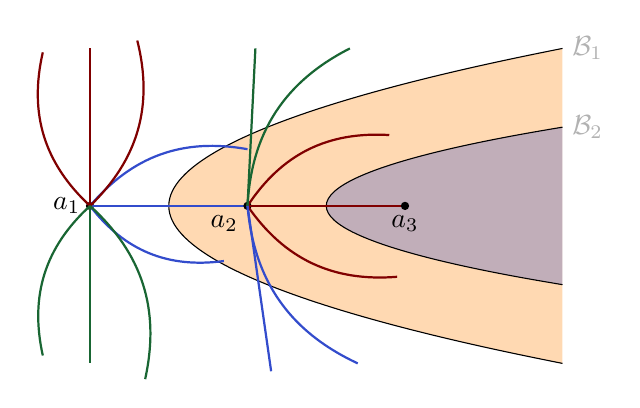
\begin{tikzpicture}[rotate=270]
      \draw [fill opacity=0.3, fill=morange] (2, 0) parabola bend (0, -5) (-2, 0) node [right] {$\mathcal{B}_1$};
      \draw [fill opacity=0.3, fill=mblue] (1, 0) parabola bend (0, -3) (-1, 0) node [right] {$\mathcal{B}_2$};

      \node [circ] at (0, -6) {};
      \node [left] at (0, -6) {$a_1$};

      \draw [thick, mblue] (0, -6) -- (0, -4);
      \draw [thick, mblue] (0, -6) edge [bend left] (-0.72, -4);
      \draw [thick, mblue] (0, -6) edge [bend right] (0.7, -4.3);

      \draw [thick, mred] (0, -6) -- (-2, -6);
      \draw [thick, mred] (0, -6) edge [bend left] (-1.95, -6.6);
      \draw [thick, mred] (0, -6) edge [bend right] (-2.1, -5.4);

      \draw [thick, mgreen] (0, -6) -- (2, -6);
      \draw [thick, mgreen] (0, -6) edge [bend right] (1.9, -6.6);
      \draw [thick, mgreen] (0, -6) edge [bend left] (2.2, -5.3);

      \node [circ] at (0, -4) {};
      \node [anchor = north east] at (0, -4) {$a_2$};

      \draw [thick, mred] (0, -4) -- (0, -2);
      \draw [thick, mred] (0, -4) edge [bend left] (-0.9, -2.2);
      \draw [thick, mred] (0, -4) edge [bend right] (0.9, -2.1);

      \draw [thick, mgreen] (0, -4) edge [bend left] (-2, -2.7);
      \draw [thick, mgreen] (0, -4) -- (-2, -3.9);

      \draw [thick, mblue] (0, -4) edge [bend right] (2, -2.6);
      \draw [thick, mblue] (0, -4) -- (2.1, -3.7);

      \node [circ] at (0, -2) {};
      \node [below] at (0, -2) {$a_3$};
    \end{tikzpicture}
  \end{center}
  We obtain a sequence $\{a_1, a_2, \cdots\}$ and a sequence of colours $\{c_1, c_2, \cdots\}$ such that $c(a_i a_j) = c_i$, for $i < j$.

  Now again by the pigeonhole principle, since there are finitely many colours, there exists an infinite subsequence $c_{i_1}, c_{i_2}, \cdots$ that is constant. Then $a_{i_1}, a_{i_2}, \cdots$ is an infinite monochromatic set, since all edges are of the colour $c_{i_1} = c_{i_2} = \cdots$. So we are done.
\end{proof}
Note that this theorem is highly non-constructive. Not only does it not give us the infinite monochromatic set; it doesn't even tell us what the colour is.

Note also that in the proof, we did not obtain the infinite monochromatic set in one go. Instead, we had to first pass through that intermediate structure, and then obtain an infinite monochromatic set from that. This is a common feature in many proofs in Ramsey theory, and in many cases we have to pass through even more intermediate substructures.

This theorem looks rather innocuous, but it has many interesting applications.
\begin{cor}[Bolzano-Weierstrass theorem]
  Let $(x_i)_{i \geq 0}$ be a bounded sequence of real numbers. Then it has a convergent subsequence.
\end{cor}

\begin{proof}
  We define a colouring $c: \N^{(2)} \to \{\uparrow, \downarrow\}$, where
  \[
    c(ij) =
    \begin{cases}
      \uparrow & x_i < x_j\\
      \downarrow & x_j \leq x_i
    \end{cases}
  \]
  Then Ramsey's theorem gives us an infinite monochromatic set, which is the same as a monotone subsequence. Since this is bounded, it must convergence.
\end{proof}

Now a natural question to ask is --- what happens when we have infinitely many colours? Clearly an infinite monochromatic subset cannot be guaranteed, because we can just colour all edges with different colours. Thus, we can ask a different question --- can we find an $X$ such that \emph{either} $c|_{X}$ is monochromatic, \emph{or} $c|_{X}$ is injective.

It turns out this is also not quite true. We can construct a colouring on $\N^{(2)}$ as follows: we first colour all edges that involve $1$ with the colour $1$, then all edges that involve $2$ with the colour $2$ etc., and then we will realize we cannot find an infinite monochromatic subset or an infinite subset with all edges of different colours. So we need to take these things into account as well.

It turns out to answer this question, we need the following natural generalization of Ramsey's theorem:
\begin{thm}[Ramsey's theorem for $r$ sets]\index{Ramsey's theorem!for $r$ sets}
  Whenever $\N^{(r)}$ is $k$-coloured, there exists an infinite monochromatic set, ie. for any $c: \N^{(r)} \to [k]$, there exists an infinite $X \subseteq \N$ such that $c|_{X^{(r)}}$ is constant.
\end{thm}

\begin{eg}
  We define $c: \N^{(3)} \to \{\mathrm{red}, \mathrm{blue}$ by
  \[
    c(ijk) =
    \begin{cases}
      \mathrm{red} & i \mid j + k\\
      \mathrm{blue} & \mathrm{otherwise}
    \end{cases}
  \]
  Then $X = \{2^0, 2^1, 2^2, \cdots\}$ is an infinite monochromatic set.
\end{eg}


\begin{proof}
  We induct on $r$. This is trivial when $r = 1$. Assume $r > 1$. We fix $a_1 \in \N$. We induce a $k$-colouring $c_1$ of $(\N \setminus \{a_1\})^{(r - 1)}$ by
  \[
    c_1(F) = c(F \cup \{a_1\}).
  \]
  By induction, there exists an infinite $B_1 \subseteq \N \setminus \{a_1\}$ such that $B_1$ is monochromatic for $c_1$, ie. all $a_1-B_1$ $r$-sets have the same colour $c_1$.

  We proceed inductively as before. We get $a_1, a_2, a_3, \cdots$ and colours $c_1, c_2, \cdots$ etc. such that for any $r$-set $F$ contained in $\{a_1, a_2, \cdots\}$, we have $c(F) = c_{\min F}$.

  Then again, there exists $c_{i_1}, c_{i_2}, c_{i_3}, \cdots$ all identical, and our monochromatic set is $\{a_{i_1}, a_{i_2}, a_{i_3}, \cdots\}$.
\end{proof}

With this, we can answer our previous question:
\begin{thm}[Canonical Ramsey theorem]\index{canonical Ramsey theorem}\index{Ramsey theorem!canonical}
  For any $c: \N^{(2)} \to \N$, there exists an infinite $X \subseteq \N$ such that one of the following hold:
  \begin{enumerate}
    \item $c|_{X^{(2)}}$ is constant.
    \item $c|_{X^{(2)}}$ is injective.
    \item $c(ij) = c(k\ell)$ iff $i = k$ for all $i, j, k \ell \in X$.
    \item $c(ij) = c(k\ell)$ iff $j = \ell$ for all $i, j, k \ell \in X$.
  \end{enumerate}
\end{thm}
Recall that when we write $ij$, we always implicitly assume $i < j$, so that (iii) and (iv) make sense.

In previous proofs, we only had to go through two passes to get the desired set. This time we will need more.
\begin{proof}
  Consider the following colouring of $X^{(4)}$: let $c_1$ be a $2$-colouring
  \[
    c_1(ijk\ell) =
    \begin{cases}
      \mathtt{SAME} & c(ij) = c(k\ell)\\
      \mathtt{DIFF} & \mathrm{otherwise}
    \end{cases}
  \]
  \begin{center}
    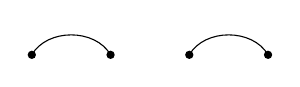
\begin{tikzpicture}
      \foreach \x in {0, 1, 2, 3} {
        \node [circ] at (\x, 0) {};
      }
      \draw (0, 0) edge [out=60, in=120] (1, 0);
      \draw (2, 0) edge [out=60, in=120] (3, 0);
    \end{tikzpicture}
  \end{center}
  Then we know there is some infinite monochromatic set $X_1 \subseteq \N$ for $c_1$. If $X_1$ is coloured $\mathtt{SAME}$, then we are done, since $c|_{X_1^{(2)}}$ is constant, since for any pair $ij$ and $i'j'$, we can pick some huge $k, \ell$ such that $j, j' < k < \ell$, and then
  \[
    c(ij) = c(k\ell) = c(i'j')
  \]
  as we know $c_1(ijk\ell) = c_1(i'j'k\ell) = \mathtt{SAME}$.

  What if $X_1$ is coloured $\mathtt{DIFF}$? We next look at what happens when we have edges that are nested each other. We define $c_2: X_1^{(4)} \to \{\mathtt{SAME}, \mathtt{DIFF}\}$ defined by
  \[
    c_2(ijk\ell) =
    \begin{cases}
      \mathtt{SAME} & c(i\ell) = c(jk)\\
      \mathtt{DIFF} & \mathrm{otherwise}
    \end{cases}
  \]
  \begin{center}
    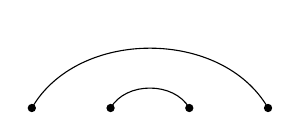
\begin{tikzpicture}
      \foreach \x in {0, 1, 2, 3} {
        \node [circ] at (\x, 0) {};
      }
      \draw (0, 0) edge [out=60, in=120] (3, 0);
      \draw (1, 0) edge [out=60, in=120] (2, 0);
    \end{tikzpicture}
  \end{center}
  Again, we can find an infinite monochromatic subset $X_2 \subseteq X_1$ with respect to $c_2$.

  We now note that $X_2$ cannot be coloured $\mathtt{SAME}$. Indeed, we can just look at
  \begin{center}
    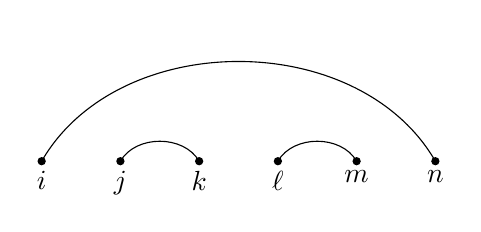
\begin{tikzpicture}
      \foreach \x/\y in {0/i, 1/j, 2/k, 3/\ell, 4/m, 5/n} {
        \node [circ] at (\x, 0) {};
        \node [below] at (\x, 0) {$\y$};
      }
      \draw (0, 0) edge [out=60, in=120] (5, 0);
      \draw (1, 0) edge [out=60, in=120] (2, 0);
      \draw (3, 0) edge [out=60, in=120] (4, 0);
    \end{tikzpicture}
  \end{center}
  So if $X_2$ were $\mathtt{SAME}$, we would have
  \[
    c(\ell m) = c(in) = c(jk),
  \]
  which is impossible since $X_1$ is coloured $\mathtt{DIFF}$ under $c_1$.

  So $X_2$ is $\mathtt{DIFF}$. Now consider $c_3: X_2^{(4)} \to \{\mathtt{SAME}, \mathtt{DIFF}\}$ given by
  \[
    c_3(ijk\ell) =
    \begin{cases}
      \mathtt{SAME} & c(ik) = c(j\ell)\\
      \mathtt{DIFF} & \mathrm{otherwise}
    \end{cases}
  \]
  \begin{center}
    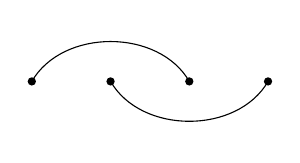
\begin{tikzpicture}
      \foreach \x in {0, 1, 2, 3} {
        \node [circ] at (\x, 0) {};
      }
      \draw (0, 0) edge [out=60, in=120] (2, 0);
      \draw (1, 0) edge [out=-60, in=-120] (3, 0);
    \end{tikzpicture}
  \end{center}
  Again find an infinite monochromatic subset $X_3 \subseteq X_2$ for $c_3$. Then $X_3$ cannot be $\mathtt{SAME}$, this time using the following picture:
   \begin{center}
    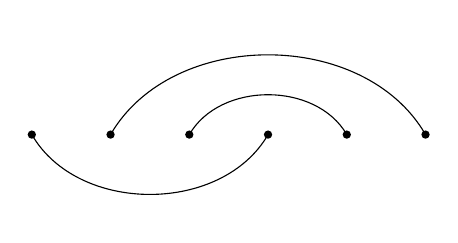
\begin{tikzpicture}
      \foreach \x/\y in {0, 1, 2, 3, 4, 5} {
        \node [circ] at (\x, 0) {};
      }
      \draw (0, 0) edge [out=-60, in=-120] (3, 0);
      \draw (1, 0) edge [out=60, in=120] (5, 0);
      \draw (2, 0) edge [out=60, in=120] (4, 0);
    \end{tikzpicture}
  \end{center}
  contradicting the fact that $c_2$ is $\mathtt{DIFF}$. So we know $X_3$ is $\mathtt{DIFF}$.

  We have now have ended up in this set $X_3$ such that if we have any two pairs of edges with different end points, then they must be different.

  We now want to look at cases where things share a vertex. Consider $c_4: X_3^{(3)} \to \{\mathtt{SAME}, \mathtt{DIFF}\}$ given by
  \[
    c_4(ijk) =
    \begin{cases}
      \mathtt{SAME} & c(ij) = c(jk)\\
      \mathtt{DIFF} & \mathrm{otherwise}
    \end{cases}
  \]
  \begin{center}
    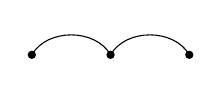
\begin{tikzpicture}
      \foreach \x in {0, 1, 2} {
        \node [circ] at (\x, 0) {};
      }
      \draw (0, 0) edge [out=60, in=120] (1, 0);
      \draw (1, 0) edge [out=60, in=120] (2, 0);
    \end{tikzpicture}
  \end{center}
  Let $X_4 \subseteq X_3$ be an infinite monochromatic set for $c_4$. Now $X_4$ cannot be coloured $\mathtt{SAME}$, using the following picture:
  \begin{center}
    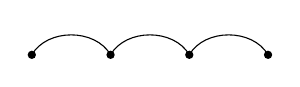
\begin{tikzpicture}
      \foreach \x in {0, 1, 2, 3} {
        \node [circ] at (\x, 0) {};
      }
      \draw (0, 0) edge [out=60, in=120] (1, 0);
      \draw (1, 0) edge [out=60, in=120] (2, 0);
      \draw (2, 0) edge [out=60, in=120] (3, 0);
    \end{tikzpicture}
  \end{center}
  which contradicts the fact that $c_1$ is $\mathtt{DIFF}$. So we know $X_4$ is also coloured $\mathtt{DIFF}$ under $c_4$.

  We are almost there. We need to deal with edges that nest in the sense of (iii) and (iv). We look at $c_5: X_4^{(3)} \to \{\mathtt{LSAME}, \mathtt{LDIFF}\}$ given by
  \[
    c_5(ijk) =
    \begin{cases}
      \mathtt{LSAME} & c(ij) = c(ik)\\
      \mathtt{LDIFF} & \mathrm{otherwise}
    \end{cases}
  \]
   \begin{center}
    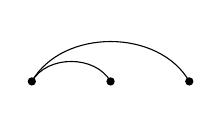
\begin{tikzpicture}
      \foreach \x in {0, 1, 2} {
        \node [circ] at (\x, 0) {};
      }
      \draw (0, 0) edge [out=60, in=120] (1, 0);
      \draw (0, 0) edge [out=60, in=120] (2, 0);
    \end{tikzpicture}
  \end{center}
  Again we find $X_5 \subseteq X_4$, an infinite monochromatic set for $c_5$. We don't separate into cases yet, because we know both cases are possible, but move on to classify the right case as well. Define $c_6: X_5^{(3)} \to \{\mathtt{RSAME}, \mathtt{RDIFF}\}$ given by
  \[
    c_5(ijk) =
    \begin{cases}
      \mathtt{RSAME} & c(ik) = c(jk)\\
      \mathtt{RDIFF} & \mathrm{otherwise}
    \end{cases}
  \]
   \begin{center}
    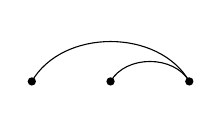
\begin{tikzpicture}
      \foreach \x in {0, 1, 2} {
        \node [circ] at (\x, 0) {};
      }
      \draw (1, 0) edge [out=60, in=120] (2, 0);
      \draw (0, 0) edge [out=60, in=120] (2, 0);
    \end{tikzpicture}
  \end{center}
  Let $X_6 \subseteq X_5$ be an infinite monochromatic subset under $c_5$.

  As before, we can check that it is impossible to get both $\mathtt{LSAME}$ and $\mathtt{RSAME}$, using the following picture:
  \begin{center}
    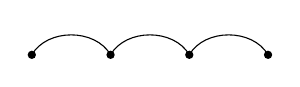
\begin{tikzpicture}
      \foreach \x in {0, 1, 2, 3} {
        \node [circ] at (\x, 0) {};
      }
      \draw (0, 0) edge [out=60, in=120] (1, 0);
      \draw (1, 0) edge [out=60, in=120] (2, 0);
      \draw (2, 0) edge [out=60, in=120] (3, 0);
    \end{tikzpicture}
  \end{center}
  contradicting $c_4$ being $\mathtt{DIFF}$.

  Then the remaining cases $(\mathtt{LDIFF}, \mathtt{RDIFF})$, $(\mathtt{LSAME}, \mathtt{RDIFF})$ and $(\mathtt{RDIFF}, \mathtt{LSAME})$ corresponds to the cases (ii), (iii) and (iv).
\end{proof}
Note that we could this theorem in one pass only, instead of six, by considering a much more complicated colouring $(c_1, c_2, c_3, c_4, c_5, c_6)$ with values in
\[
  \{\mathtt{SAME}, \mathtt{DIFF}\}^4 \times \{\mathtt{LSAME}, \mathtt{LDIFF}\} \times \{\mathtt{RSAME}, \mathtt{RDIFF}\},
\]
but we still have to do the same analysis and it just complicates matters more.

There is a generalization of this to $r$-sets. One way we can rewrite the theorem is to say that the colour is uniquely determined by some subset of the vertices. The cases (i), (ii), (iii), (iv) correspond to no vertices, all vertices, first vertex, and second vertex respectively. Then for $r$-sets, we have $2^r$ possibilities, one for each subset of the $r$-coordinates.

\begin{thm}[Higher dimensional canonical Ramsey theorem]\index{higher dimensional canonical Ramsey theorem}\index{canonical Ramsey theorem!!higher dimensional}\index{Ramsey theorem!higher dimensional, canonical}
  Let $c: \N^{(r)} \to \N$ be a colouring. Then there exists $D \subseteq [r]$ and an infinite subset $X \subseteq \N$ such that for all $x \not= y \in X^{(r)}$, we have $c(x) = c(y)$ iff $\{i: x_i = y_i\} = D$, where $x = \{x_1 < x_2 < \cdots < x_r\}$ (and similarly for $y$).
\end{thm}

\subsection{Finite graphs}
We will usually restrict to $2$ colours. Everything we say will either be trivially be generalizable to more colours, or we have no idea how to do so. It is an exercise for the reader to figure out which it is.

Recall again that a graph $G$ is a pair $(V, E)$ where $E \subseteq V^{(2)}$.
\begin{eg}
  The \term{path graph} on $n$ vertices \term{$P_n$} is
  \begin{center}
    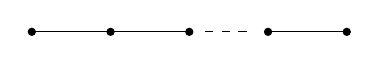
\begin{tikzpicture}
      \draw (0, 0) node [circ] {} -- (1, 0) node [circ] {} -- (2, 0) node [circ] {};

      \draw [dashed] (2.2, 0) -- (2.8, 0);

      \draw (3, 0) node [circ] {} -- (4, 0) node [circ] {};
    \end{tikzpicture}
  \end{center}
  We can write
  \[
    V = [n],\quad E = \{12, 23, 34, \cdots, (n-1)n\}.
  \]
\end{eg}

\begin{eg}
  The $n$-cycle \term{$C_n$} is
  % insert picture
  \[
    V = [n],\quad E = \{12, 23, \cdots, (n-1)n, 1n\}.
  \]
\end{eg}

Finally, we have
\begin{eg}
  The \term{complete graph} \term{$V_n$} on $n$ vertices is
  \[
    V = [n], E = V^{(2)}.
  \]
\end{eg}

Our previous Ramsey theorem can be said as saying given an infinite complete graph $K_n$ with a colouring, there is an infinite monochromatic complete subgraph.

Obviously, our initial graph had to be infinite for the result to hold. But we can ask another question --- how big does our graph have to be to guarantee a complete monochromatic subgraph of size $n$?
\begin{defi}[Ramsey number]\index{Ramsey number}\index{$R(n)$}\index{$R(K_n)$}
  We let $R(n) = R(K_n)$ to be the smallest $N \in \N$ whenever we red-blue colour the edges of $K_N$, then there is a monochromatic copy of $K_n$.
\end{defi}

\begin{thm} % insert name
  For all $n$, we have $R(n) < \infty$.
\end{thm}

\begin{proof}
  Suppose not. Let $n$ be such that $R(n) = \infty$. Then for any $m \geq n$, there is a $2$-colouring $c_m$ of $K_m = [m]^{(2)}$ such that there is no monochromatic et of size $n$.

  We want to use these colourings to build up a colouring of $\N^{(2)}$ with no monochromatic set of size $n$. We want to say we take the ``limit'' of these colourings, but what does this mean? To do so, we need these colourings to be nested.

  By the pigeonhole principle, there exists an infinite set $M_1 \subseteq \N$ and some fixed $2$-colouring $d_n$ of $[n]$ such that $c_m|_{[n]^{(2)}} = d_n$ for all $m \in M_1$.

  Similarly, there exists an infinite $M_2 \subseteq M_1$ such that $c_m|_{[n + 1]^{(2)}} = d_{n + 1}$ for $m \in M_2$, again for some $2$-colouring $d_{n + 1}$ of $[n + 1]$. We repeat this over and over again. Then we get a sequence $d_n, d_{n + 1}, \cdots$ of colourings such that $d_i$ is a $2$-colouring of $[i]^{(2)}$ without a monochromatic $K_n$, and further for $i < j$, we have
  \[
    d_j|_{[i]^{(2)}} = d_i.
  \]
  We then define a $2$-colouring $c$ of $\N^{(2)}$ by
  \[
    c(ij) = d_m(ij)
  \]
  for any $m > i, j$. Clearly, there exists no monochromatic $K_n$ in $c$, as any $K_n$ is finite. This massively contradicts the infinite Ramsey theorem.
\end{proof}
There are other ways of proving this. We can do it by using compactness. We consider the space $\{1, 2\}^\N$ with metric
\[
  d(f, g) = \frac{1}{2^n}\text{ if } n = \min \{i: f_i \not= g_i\}.
\]
By Tychonoff theorem, we know this is compact, and we can deduce the theorem from this. % how?

The problem with these proofs is that they are completely non-constructive. The proof gives us no bound on $R(n)$ whatsoever.

To obtain a bound, we can mimic the proof of the infinite Ramsey theorem. To do so, it is convenient to consider the following generalization of the Ramsey number: % we might have found a lot of blue things, and we want a big red or small blue.
\begin{defi}[Off-diagonal Ramsey number]\index{off-diagonal Ramsey number}\index{Ramsey number!off-diagonal}\index{$R(n, m)$}\index{$R(K_n, K_m)$}
  We define $R(n, m) = R(K_n, K_m)$ to be the minimum $N \in \N$ such that whenever we red-blue colour the edges of $K_N$, we either get a red $K_n$ or a blue $K_m$.
\end{defi}

Clearly we have
\[
  R(n, m) \leq R(\max{n, m}).
\]
In particular, they are finite. Once we make this definition, it is easy to find an easy bound on $R$.
\begin{thm}
  We have
  \[
    R(n, m) \leq R(n - 1, m) + R(n, m - 1).
  \]
  for all $n, m \in \N$. Consequently, we have
  \[
    R(n, m) \leq \binom{n + m - 1}{n - 2}.
  \]
\end{thm}

\begin{proof}
  We induct on $n + m$. It is clear that
  \[
    R(1, n) = R(n, 1) = 1,\quad R(n, 2) = R(2, n) = n
  \]
  Now suppose $N \geq R(n - 1, m) + R(n, m - 1)$. Consider any red-blue colouring of $K_N$ and any vertex $v \in V(K_n)$. We write
  \[
    v(K_n) \setminus \{v\} = A \cup B,
  \]
  where each vertex $A$ is joined by a red edge to $v$, and each vertex in $B$ is joined by a blue edge to $v$. Then
  \[
    |A| + |B| \geq N - 1 \geq R(n - 1, m) + R(n, m - 1) - 1.
  \]
  It follows that either $|A| \geq R(n - 1, m)$ or $|B| \geq R(n, m - 1)$. We wlog it is the former. Then by definition of $R(n - 1, m)$, we know $A$ contains either a blue copy of $K_m$ or a red copy of $K_{n - 1}$. In the first case, we are done, and in the second case, we just add $v$ to the red $K_{n - 1}$.

  The last formula is just a straightforward property of binomial coefficients.
\end{proof}

In particular, we find
\[
  R(n) \leq \binom{2n - 1}{n - 2} \leq \frac{4^n}{\sqrt{n}}.
\]
We genuinely have no idea whether $\sim 4^n$ is the correct growth rate, ie. if there is some $\varepsilon$ such that $R(n) \leq (4 - \varepsilon)^n$. However, we do know that
\[
  R(n) \leq \frac{4^n}{n^c}
\]
for any $c > 0$ (eventually).

But do we have a lower bound? Does it have to grow exponentially? The answer is yes, and the answer is a very classical construction of Erd\"os.

\begin{thm}
  We have $R(n) \geq \sqrt{2}^n$ for sufficiently large $n \in \N$.
\end{thm}
The proof is remarkable in that before this was shown, we had no sensible bound at all. However, the proof is incredibly simple, and revolutionized how we think about colourings.

\begin{proof}
  Let $N \leq \sqrt{2}^N$. We perform a red-blue colouring of $K_N$ randomly, where each edge is coloured red independently of the others with probability $\frac{1}{2}$.

  We let $X_R$ be the number of red copies of $K_n$ in such a colouring. Then since expectation is linear, we know the expected value is
  \begin{align*}
    [X_R] &= \binom{N}{n} \left(\frac{1}{2}\right)^{-\binom{n}{2}}\\
    &\leq \left(\frac{eN}{n}\right)^n \left(\frac{1}{2}\right)^{\binom{n}{2}}\\
    &\leq \left(\frac{e}{n}\right)^n \sqrt(2)^{n^2} \sqrt{2}^{-n^2}\\
    &= \left(\frac{e}{n}\right)^{n}\\
    &< \frac{1}{2}
  \end{align*}
  for sufficiently large $n$.

  Similarly, we have $[X_B] < \frac{1}{2}$. So the expected number of monochromatic $K_n$ is $< 1$. So in particular there must be some colouring with no monochromatic $K_n$.
\end{proof}

Recall the bound
\[
  R(m, n) \leq \binom{m + n - 2}{m - 1}.
\]
If we think of $m$ as being fixed, then this tells us
\[
  R(m, n) \sim (n + m)^{m - 1}.
\]
For example, if $m$ is $3$, then we have
\[
  R(3, n) \leq \binom{n + !}{2} = \frac{n(n + 1)}{2} \sim n^2.
\]
We can sort-of imagine where this bound came from. Suppose we randomly pick a vertex $v_1$. Then if it is connected to at least $n$ other vertices by a red edge, then we are done --- if there is even one red edge among those $n$ things, then we have a red triangle. Otherwise, all edges are blue, and we've found a complete blue $K_n$.

So this is connected to at most $n - 1$ things by a red edge. So if our graph is big enough, we can pick some $v_2$ connected to $v_1$ by a blue edge, and do the same thing to $v_2$. We keep going on, and by the time we reach $v_n$, we would have found $v_1, \cdots, v_n$ all connected to each other by blue edges, and we are done. So we have $K(3, n) \sim n^2$.

But this argument is rather weak, because we didn't use that large pool of blue edges we've found at $v_1$. So in fact this time we can do better than $n^2$.
\begin{thm}
  We have
  \[
    R(3, n) \leq \frac{100 n^2}{\log n}
  \]
  for sufficiently large $n \in \N$.
\end{thm}
Here the $100$ is, obviously, just some random big number.

\begin{proof}
  Let $N \geq 100n^2/\log n$, and consider a red-blue colouring of the edges of $K_N$ with no red $K_3$. We want to find a blue $K_n$ in such a colouring.

  We may assume that
  \begin{enumerate}
    \item No vertex $v$ has $ \geq n$ red edges incident to it, as argued just now.
    \item If we have $v_1, v_2, v_3$ such that $v_1v_2$ and $v_1 v_3$ are red, then $v_2 v_3$ is blue:
      \begin{center}
        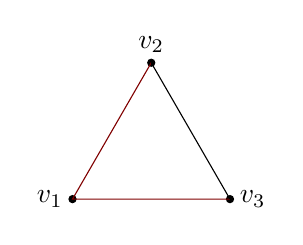
\begin{tikzpicture}
          \node [circ] at (0, 0) {};
          \node [circ] at (2, 0) {};
          \node [circ] at (1, 1.732) {};
          \draw [mred] (2, 0) -- (0, 0) -- (1, 1.732);
          \draw (1, 1.732) -- (2, 0);

          \node [left] at (0, 0) {$v_1$};
          \node [above] at (1, 1.732) {$v_2$};
          \node [right] at (2, 0) {$v_3$};
        \end{tikzpicture}
      \end{center}
  \end{enumerate}
  We now let
  \[
    \mathcal{F} = \{\mathcal{U} : \mathcal{U} \subseteq V(K_N)\text{ such that }\mathcal{U}^{(2)} \text{ is monochromatic and blue}\}.
  \]
  We want to find some $\mathcal{U} \in \mathcal{F}$ such that $|\mathcal{U}| \geq n$, ie. a blue $K_n$. How can we go about finding this?

  Let $W$ be a uniformly random member of $\mathcal{F}$. We will be done if we can show that that $\E[|W|] \geq n$.

  We are going to define a bunch of random variables. For each vertex $v \in V(K_N)$, we define the variable
  \[
    X_v = n \mathbf{1}_{\{v \in W\}} + |\{u: uv\text{ is red and }u \in W\}|.
  \]
  \begin{claim}
   \[
    \E[X_v] > \frac{\log n}{10}
  \]
  for each vertex $v$.
  \end{claim}
  To see this, let
  \[
    A = \{u: uv \text{ is red}\}
  \]
  and let
  \[
    B = \{u: uv \text{ is blue}\}.
  \]
  then from the properties we've noted down, we know that $|A| < n$ and $A^{(2)}$ is blue. So we know very well what is happening in $A$, and nothing about what is in $B$.

  We fix a set $\mathcal{S} \subseteq B$ such that $\mathcal{S} \in \mathcal{F}$, ie. $\mathcal{S}^{(2)}$ is blue. What can we say about $W$ if we condition on $B \cap W = S$?

  Let $T \subseteq A$ be the set of vertices that are joined to $S$ only by blue edges. Write $|T| = x$. Then if $B \cap W = S$, then either $W \subseteq S \cup T$, or $W \subseteq S \cup \{v\}$. So there are exactly $2^x + 1$ choices of $W$. So we know
  \begin{align*}
    \E[X_v \mid W \cap B = S] &\geq \frac{n}{2^x + 1} + \frac{2^x}{2^x + 1}(\E[\text{random subset of T}])\\
    &= \frac{n}{2^x + 1} + \frac{2^{x - 1}x}{2^x + 1}.
  \end{align*}
  Now if
  \[
    x < \frac{\log n}{2},
  \]
  then
  \[
    \frac{n}{2^x + 1} \geq \frac{n}{\sqrt{n} + 1} \geq \frac{\log n}{10}
  \]
  for all sufficiently large $n$. On the other hand, if
  \[
    x \geq \frac{\log n}{2},
  \]
  then
  \[
    \frac{2^{x - 1}x}{2^x + 1} \geq \frac{1}{4} \cdot \frac{\log n}{2} \geq \frac{\log n}{10}.
  \]
  So we are done.

  \begin{claim}
    \[
      \sum_{v \in V} X_v \leq 2n |W|.
    \]
  \end{claim}
  To see this, for each vertex $v$, we know that if $v \in W$, then it contributes $n$ to the sum via the first term. Also, by our initial observation, we know that $v \in W$ has at most $n$ neighbours. So it contributes at most $n$ to the second term (acting as the ``$u$''). So finally, we know that
  \[
    \E[|W|] \geq \frac{1}{2n} \sum \E[X_V] \geq \frac{N}{2n} \frac{\log n}{10} \geq \frac{100n^2}{\log n} \cdot \frac{\log n}{20 n} \geq 5n.
  \]
  Therefore we can always find some $\mathcal{U} \in \mathcal{F}$ such that $|\mathcal{U}| \geq n$.
\end{proof}

Now of course, there is the following obvious generalization of Ramsey numbers:
\begin{defi}[$R(G, H)$]\index{$R(G, H)$}
  Let $G, H$ be graphs. Then we define $R(G, H)$ to be the smallest $N$ such that any red-blue colouring of $K_N$ has either a red copy of $G$ or a blue copy of $H$.
\end{defi}
Obviously, we have $R(G, H) \leq R(|G|, |H|)$. So the natural question is if we can do better than that.

\begin{ex}
  Show that
  \[
    R(P_n. P_n) \leq 2n.
  \]
\end{ex}
So sometimes it cna be much better.

\section{Ramsey theory on the integers}
So far, we've been talking about what happens when we finitely colour graphs. What if we $k$-colour the integers $\N$? What can we say about it?

It is a trivial statement that this colouring has a monochromatic subset, by the pigeonhole principle. Interesting questions arise when we try to take the additive structure of $\N$ into account. So we could ask, can we find a monochromatic ``copy'' of $\N$.

One way to make this question concrete is to ask if there is an infinite monochromatic arithmetic progression.

The answer is easily a ``no''! There are only countably many progressions, so for each arithmetic progression, we pick two things in the progression and colour them differently.

We can also construct this more concretely. We can colour the first number red, the next two blue, the next three red etc. then it is easy to see that it doesn't have an infinite arithmetic progression. % insert picture

But this is somewhat silly, because there is a significant amount of structure in the sequence there. It turns out the following is true:
\begin{thm}[van der Waerden theorem]\index{van der Waerden theorem}
  Let $m, k \in N$. Then there is some $N = W(m, k)$ such that whenever $[N]$ is $k$-coloured, then there is a monochromatic arithmetic progression of length $n$.
\end{thm}

The idea is to do induction on $m$. We will using colourings with much greater than $k$ colours to deduce the existence of $W(m, k)$.

We can try a toy example first. Let's try to show that $W(3, 2)$ exists. Suppose we have three natural numbers:
\begin{center}
  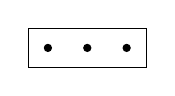
\begin{tikzpicture}[scale=0.5]
    \draw (-0.5, 0.5) rectangle (2.5, -0.5);
    \node [circ] at (0, 0) {};
    \node [circ] at (1, 0) {};
    \node [circ] at (2, 0) {};
  \end{tikzpicture}
\end{center}
By the pigeonhole principle, there must be two things that are the same colour, say
\begin{center}
  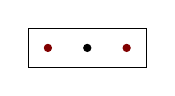
\begin{tikzpicture}[scale=0.5]
    \draw (-0.5, 0.5) rectangle (2.5, -0.5);
    \node [circ, mred] at (0, 0) {};
    \node [circ] at (1, 0) {};
    \node [circ, mred] at (2, 0) {};
  \end{tikzpicture}
\end{center}
If this is the case, then if we don't want to have an arithmetic progression of length $3$, then the fifth number must be blue
\begin{center}
  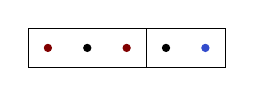
\begin{tikzpicture}[scale=0.5]
    \draw (-0.5, 0.5) rectangle (2.5, -0.5);
    \node [circ, mred] at (0, 0) {};
    \node [circ] at (1, 0) {};
    \node [circ, mred] at (2, 0) {};

    \draw (2.5, -0.5) rectangle (4.5, 0.5);
    \node [circ] at (3, 0) {};
    \node [circ, mblue] at (4, 0) {};
  \end{tikzpicture}
\end{center}
We now cut the universe into blocks into 5 things. Again by the pigeonhole principle, there must be two blocks that look the same. Say it's this block again.
\begin{center}
  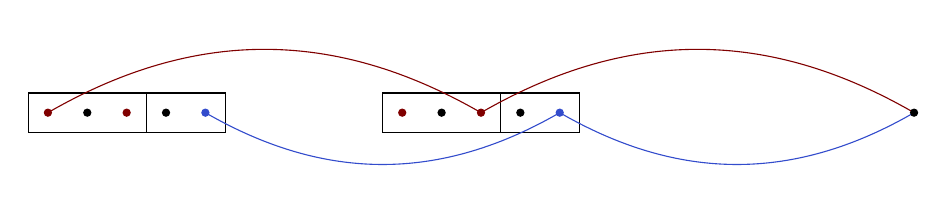
\begin{tikzpicture}[scale=0.5]
    \draw (-0.5, 0.5) rectangle (2.5, -0.5);
    \node [circ, mred] at (0, 0) {};
    \node [circ] at (1, 0) {};
    \node [circ, mred] at (2, 0) {};

    \draw (2.5, -0.5) rectangle (4.5, 0.5);
    \node [circ] at (3, 0) {};
    \node [circ, mblue] at (4, 0) {};

    \begin{scope}[shift={(9, 0)}]
      \draw (-0.5, 0.5) rectangle (2.5, -0.5);
      \node [circ, mred] at (0, 0) {};
      \node [circ] at (1, 0) {};
      \node [circ, mred] at (2, 0) {};

      \draw (2.5, -0.5) rectangle (4.5, 0.5);
      \node [circ] at (3, 0) {};
      \node [circ, mblue] at (4, 0) {};
    \end{scope}
    \draw [mred] (0, 0) edge [bend left] (11, 0);
    \draw [mred] (11, 0) edge [bend left] (22, 0);

    \draw [mblue] (4, 0) edge [bend right] (13, 0);
    \draw [mblue] (13, 0) edge [bend right] (22, 0);

    \node [circ] at (22, 0) {};
  \end{tikzpicture}

\end{center}
Now we have two sequences, and the point at the end belongs to both of the two sequences. And no matter what colour it is, we are done.

For $k = 3$, we can still find such a block, but now that third point could be a third colour, say, green. When then find these bigger blocks, and it must repeat, and then we are done again.

In the case $m = 2$, we used the pigeonhole principle. When we have $m > 2$, we will use van der Waerden theorem for smaller $m$ inductively.

We now come up with names to describe the scenario we had above.
\begin{defi}[Focused progression]
  We say a collection of arithmetic progressions $A_1, A_2, \cdots, A_r$ of length $m$ with
  \[
    A_i = \{a_i, a_i + d_i, \cdots, a_i + (m - 1) d_i\}
  \]
  are \emph{focused} at $f$ if $a_i + m d_i = f$ for all $1 \leq i \leq r$.
\end{defi}

\begin{eg}
  $\{1, 4\}$ and $\{5, 6\}$ are focused at $7$.
\end{eg}

\begin{defi}[Colour focused progression]
  If $A_1, \cdots, A_r$ are focused at $f$, and each $A_i$ is monochromatic and no two are the same colour, then we say they are \emph{colour focused} at $f$.
\end{defi}

We can now write the proof
\begin{proof}
  We induct on $m$. The result is clearly trivial when $m = 1$, and follows easily from the pigeonhole principle when $m = 2$.

  Suppose $m > !$, and assume inductively that $W(m - 1, k')$ exists for any $k' \in \N$.

  Here is the claim we are trying to established:
  \begin{claim}
    For each $r \leq k$, there is a natural number $n$ such that whenever we $k$-colour $[n]$, then either
    \begin{enumerate}
      \item There exists a monochromatic AP of length $m$; or
      \item There are $r$ colour-focused AP's of length $m - 1$.
    \end{enumerate}
  \end{claim}
  It is clear that this claim implies the theorem, as we can pick $r = k$. Then if there isn't a monochromatic AP of length $m$, then we look at the colour of the common focus, and it must be one of the colours of those AP's.

  To prove the claim, we induct on $r$. When $n = 1$, we may take $W(m - 1, k)$. Now suppose $r > 1$, and some $n'$ works for $r - 1$. With the benefit of hindsight, we shall show that
  \[
    n = W(m - 1, k^{2n'}) 2n'
  \]
  works for $r$.

  We consider any $k$-colouring of $[n]$, and suppose it has no monochromatic AP of length $m$. We need to find $r$ colour-focused progressions of length $n - 1$.

  We view this $k$-colouring of $[n]$ as a $k^{2n'}$ colouring of blocks of length $2n'$, of which there are $W(m - 1, k^{2n'})$.

  Then by definition of $W(m - 1, k^{2n'})$, we can find blocks
  \[
    B_s, B_{s + t}, \cdots, B_{s + (m - 2)t}
  \]
  which are coloured identically. By the inductive hypothesis, we know each $B_s$ contains $r - 1$ colour-focused AP's of length $m - 1$, say $A_1, .., A_{r - 1}$ with first terms $a_1, \cdots, a_r$ and common difference $d_1 , \cdots, d_{r - 1}$, and also their focus $f$, because the length of $B_s$ is $2n'$, not just $n'$.

  Since we assumed there is no monochromatic progression of length $n$, we can assume $f$ has a different colour than the $A_i$.

  Now consider $A_1', A_2', \cdots, A_{r - 1}'$, where $A_i'$ has first term $a_i$, common difference $d_i + 2n't$, and length $m - 1$. This difference sends us to the next block, and then the next term in the AP. We also pick $A_r'$ to consist of the all the focus of the blocks $B_i$, namely
  \[
    A_r' = \{f, f + 2n't, \cdots, f + 2n't(m - 2)\}
  \]
  These progressions are monochromatic with distinct colours, and focused at $f + (2n' t)(m - 1)$. So we are done.
\end{proof}

This argument, where one looks at the induced colourings of blocks, is called a \term{product argument}.

The bounds we obtain from this argument is, as one would expect, terrible. We have
\[
  W(3, k) \leq k^{\iddots^k}, % check
\]
where the tower of $k$'s has length $k$.

Instead of an arithmetic progression, why don't we ask for something that looks like $\{d, 2d, 3d, \cdots, nd\}$? This is answered on the example sheet.
\section{Partition Regularity}
\section{Topological Dynamics}

\printindex
\end{document}
